\documentclass{article}
\usepackage[T1]{fontenc}
\usepackage{lmodern}
\usepackage{graphicx}
\usepackage{amsmath,amssymb}
\usepackage[a4paper,margin=2cm]{geometry}
\usepackage[absolute,overlay]{textpos}
\setlength{\TPHorizModule}{1mm}
\setlength{\TPVertModule}{1mm}
\usepackage[indonesian]{babel}
\usepackage{hyperref}
\setlength{\emergencystretch}{2em}
% unit: Halaman 46

\begin{document}

% === Halaman 46 (llm) ===

\section*{Program enkripsi-dekripsi AES dengan Python}
\textbf{Input: Teks dari keyboard}

\vspace{167.21mm}

\begin{verbatim}
from Crypto.Cipher import AES
from Crypto.Random import get_random_bytes
from Crypto.Util.Padding import pad, unpad
import base64

# Panjang blok AES
BLOCK_SIZE = 16

def enkripsi_aes(plainteks, kunci):
    kunci = kunci.encode()
    iv = get_random_bytes(BLOCK_SIZE)
    AEScipher = AES.new(kunci, AES.MODE_CBC, iv)

    plainteks = pad(plainteks.encode(), BLOCK_SIZE)

    cipherteks = AEScipher.encrypt(plainteks)
    cipherteks = base64.b64encode(iv+cipherteks)
    return cipherteks
\end{verbatim}

% deskripsi: Screenshot cuplikan kode Python untuk fungsi enkripsi AES menggunakan library PyCryptodome
% bbox normalisasi: [0.0480, 0.2310, 0.8900, 0.7940]
\begin{textblock*}{176.82mm}(10.08mm,68.61mm)
\noindent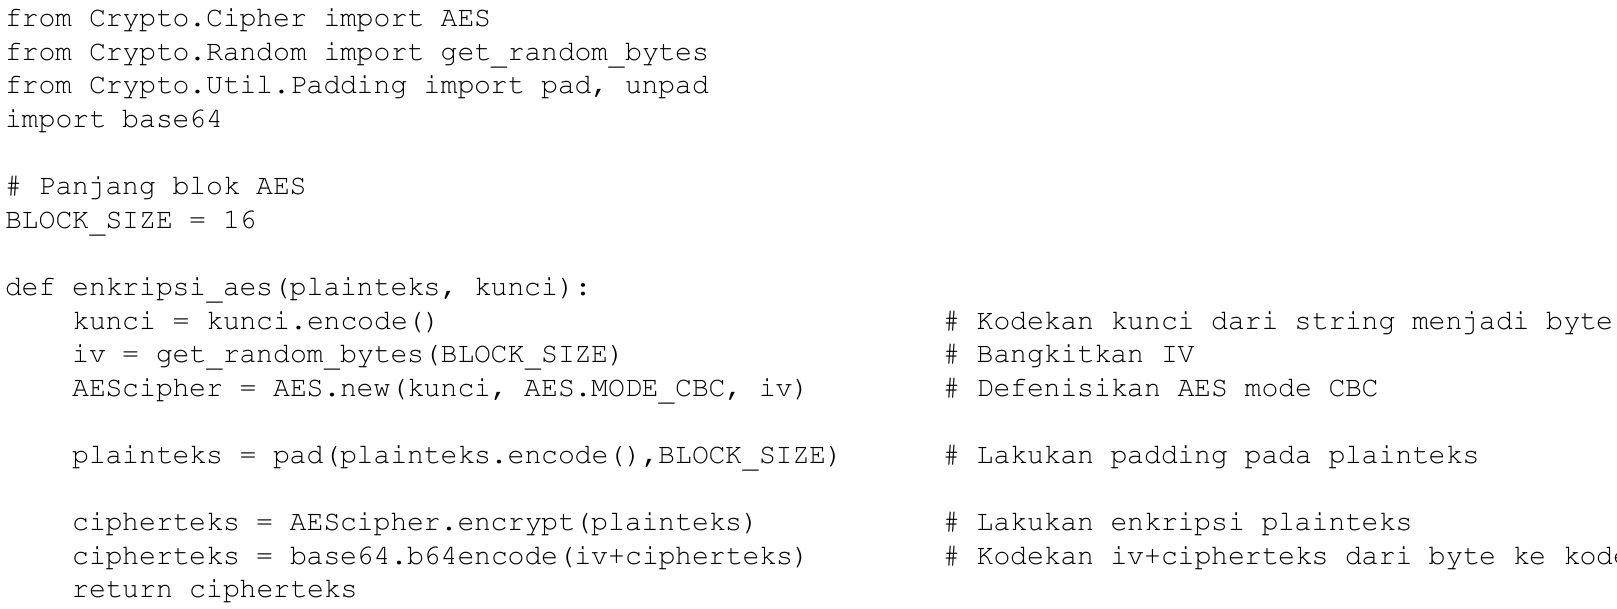
\includegraphics[width=176.82mm,height=167.21mm]{../../images/llm/page_046_img_01.png}%
\end{textblock*}

\end{document}
